\documentclass{article}
\usepackage[utf8]{inputenc}
\usepackage{tikz,pgfplots}
\usetikzlibrary{positioning}
\usetikzlibrary {intersections}
\usetikzlibrary {shapes.symbols}
\usetikzlibrary{backgrounds}

% \title{TikZPrac}
% \author{Galaxy Being}
% \date{December 2022}

\begin{document}

%\maketitle


%\section{Introduction}

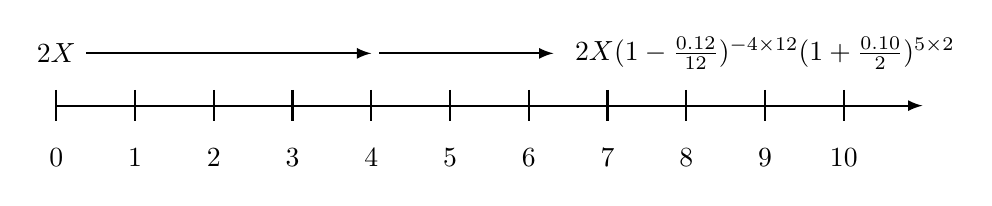
\begin{tikzpicture}[thick,time/.style={minimum height=5mm,minimum width=6mm,fill=#1,text=black},
  % every node/.style={draw},
  ]
  \draw[black,-latex] (0,0)--(11,0);
  \def\dx{1}
  \foreach \i in {0,...,10} {
    \ifnum\i>0
      \def\ann{$ $}
    \else
      \def\ann{$ 2X$}
    \fi
    \draw[] (\i*\dx,.2) -- (\i*\dx,-.2)
    node[pos=0,above=2mm,time=white] (P\i) {\ann}
    node[pos=1,below=2mm,time=white] (Q\i) {$\i$};
  }
  \node[time=white] at (P9) (x) {$2X(1-\frac{0.12}{12})^{-4\times12}(1+\frac{0.10}{2})^{5\times2} $};
  \draw[-latex] (P0)--(P4.center);
  \draw[-latex] ([xshift=1mm]P4.center)--(P6.east);
\end{tikzpicture}

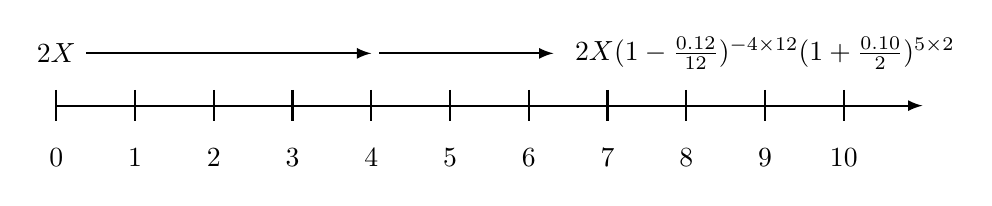
\begin{tikzpicture}[thick,time/.style={minimum height=5mm,minimum width=6mm,fill=#1,text=black},
  % every node/.style={draw},
  ]
  \draw[black,-latex] (0,0)--(11,0);
  \def\dx{1}
  \foreach \i in {0,...,10} {
    \ifnum\i>0
      \def\ann{$ $}
    \else
      \def\ann{$ 2X$}
    \fi
    \draw[] (\i*\dx,.2) -- (\i*\dx,-.2)
    node[pos=0,above=2mm,time=white,fill=none] (P\i) {\ann}
    node[pos=1,below=2mm,time=white,fill=none] (Q\i) {$\i$};
  }
  \node[time=white,fill=none] at (P9) (x) {$2X(1-\frac{0.12}{12})^{-4\times12}(1+\frac{0.10}{2})^{5\times2} $};
  \draw[-latex] (P0)--(P4.center);
  \draw[-latex] ([xshift=1mm]P4.center)--(P6.east);
\end{tikzpicture}


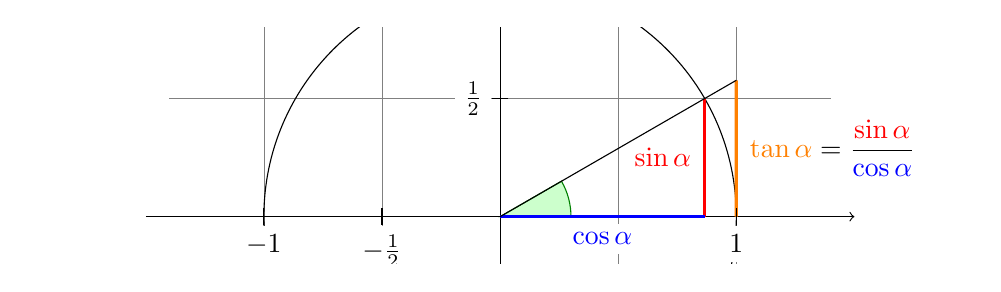
\begin{tikzpicture}[scale=3]
  \clip (-2,-0.2) rectangle (2,0.8);
  \draw[step=.5cm,gray,very thin] (-1.4,-1.4) grid (1.4,1.4);
  \filldraw[fill=green!20,draw=green!50!black] (0,0) -- (3mm,0mm)
  arc [start angle=0, end angle=30, radius=3mm] -- cycle;
  \draw[->] (-1.5,0) -- (1.5,0) coordinate (x axis);
  \draw[->] (0,-1.5) -- (0,1.5) coordinate (y axis);
  \draw (0,0) circle [radius=1cm];

  \draw[very thick,red]
  (30:1cm) -- node[left=1pt,fill=white] {$\sin \alpha$} (30:1cm |- x axis);
  \draw[very thick,blue]
  (30:1cm |- x axis) -- node[below=2pt,fill=white] {$\cos \alpha$} (0,0);
  \path [name path=upward line] (1,0) -- (1,1);
  \path [name path=sloped line] (0,0) -- (30:1.5cm);
  \draw [name intersections={of=upward line and sloped line, by=t}]
  [very thick,orange] (1,0) -- node [right=1pt,fill=white]
  {$\displaystyle \tan \alpha \color{black}=
    \frac{{\color{red}\sin \alpha}}{\color{blue}\cos \alpha}$} (t);

  \draw (0,0) -- (t);

  \foreach \x/\xtext in {-1, -0.5/-\frac{1}{2}, 1}
  \draw (\x cm,1pt) -- (\x cm,-1pt) node[anchor=north,fill=white] {$\xtext$};
  \foreach \y/\ytext in {-1, -0.5/-\frac{1}{2}, 0.5/\frac{1}{2}, 1}
  \draw (1pt,\y cm) -- (-1pt,\y cm) node[anchor=east,fill=white] {$\ytext$};
\end{tikzpicture}


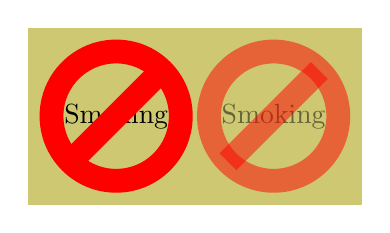
\begin{tikzpicture}[background rectangle/.style={fill=olive!45}, show background rectangle]
  \node at (0,0) [forbidden sign,line width=2ex,draw=red,fill=none] {Smoking};

  \node [opacity=.5]
        at (2,0) [forbidden sign,line width=2ex,draw=red,fill=none] {Smoking};
\end{tikzpicture}


\end{document}